% !TEX root = ../report.tex

\clearpage
\chapter{Pattern Documentation}
\label{ch:patterns}


\section{Core}
\subsection{Layers}
% see https://www.docker.com/sites/default/files/what-is-vm-diagram.png

\subsection{Client Server}
% see https://docs.docker.com/engine/introduction/understanding-docker/
% also nice image we can borrow: https://docs.docker.com/engine/article-img/architecture.svg
\begin{figure}[H]
\caption{An overview of the Docker architecture, showing the client and daemon. Source: \cite{dockerarchi}.}
\centering
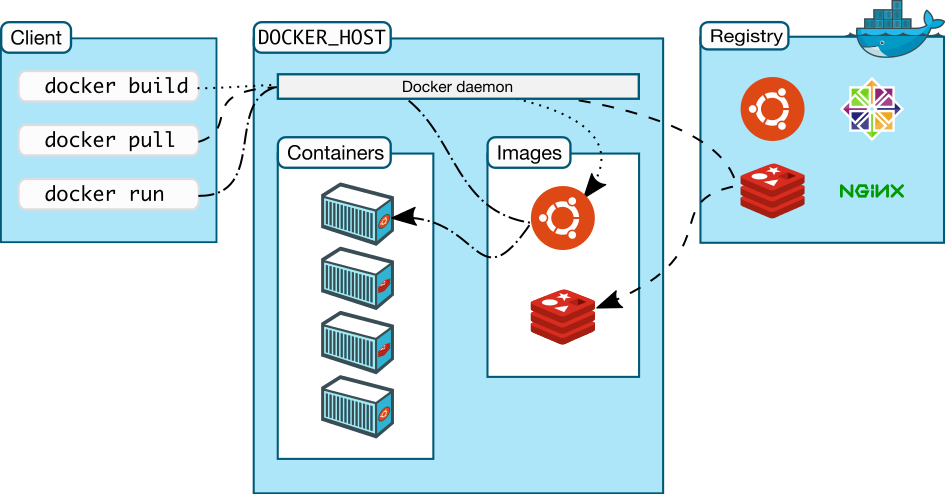
\includegraphics[scale=0.4]{4-softwarearch/images/architecture.png}
\end{figure}

\begin{description}
\item [Traceability]~\\


\item [Source]~\\


\item [Issue]~\\


\item [Assumptions/Constraints]~

\item [Solution]~


\item [Rationale] ~\\

\item [Implications]~\\


\item [Related Patterns]~\\


\end{description}

\subsection{Shared repository}
Can we consider the docker registry a shared repository?




\section{Modules}
\subsection{Interceptor}
\subsection{Plugin}

